\documentclass{article}

\usepackage{graphicx}
\usepackage[a4paper, portrait, margin=2cm]{geometry}

\renewcommand{\familydefault}{\sfdefault}
\graphicspath{ {./images/} } 

\title{Bedienungsanleitung DMX-LED-Bar}
\author{Robin Marty}
\date{25.07.2024}

\begin{document}
\maketitle
\pagenumbering{gobble}
\newpage
\pagenumbering{arabic}
\section {System Übersicht}
Eine DMX-LED-Bar besteht aus zwei Teilen: Der LED-Bar selbst und einer Anschluss-Box.

\subsection{LED-Bar}
Auf einer 2m langen LED-Bar befinden sich 120 einzeln adressierbare RGB LED Pixel. Der einzige Anschuss an der Bar selbst führt über ein 2m langes Kabel an die Anschluss-Box.\\
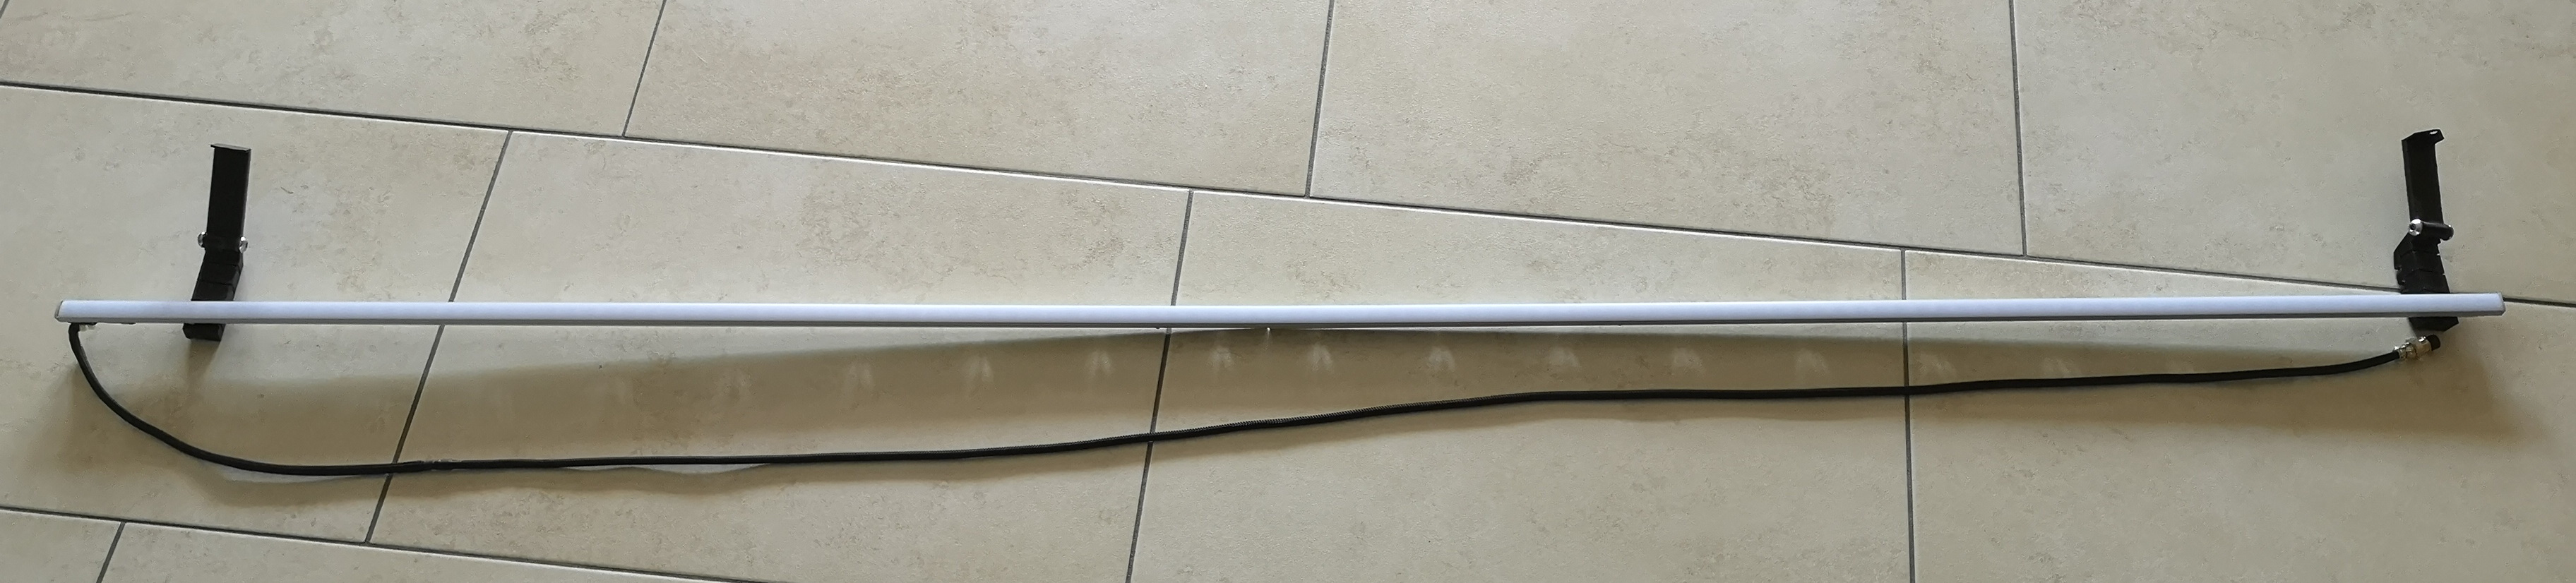
\includegraphics[width = \textwidth]{LED-Bar}

\subsection{Anschluss-Box}
In der Anschluss-Box ist die gesamte Steuerungs-Elektronik, Stromversorgung und alle weiterführenden Anschlüsse enthalten. Für den Anschluss an ein DMX Netzwerk ist eine Männliche 3-Pol XLR Buchse als Input und eine Weibliche 3-Pol XLR Buchse als Output verbaut.\\
Für die Stromversorgung ab einem 230V 50Hz Netz\textsuperscript{1}, sind eine C14 Buchse als Eingang und eine C13 Buchse als Ausgang enthalten. Die internen Verbindungen sind so ausgelegt, dass ein Strom von 10A durchgeschlauft werden kann.\\
Der Letze Anschuss (oben mitig) wird für die Verbindung zur LED-Bar genutzt.\\
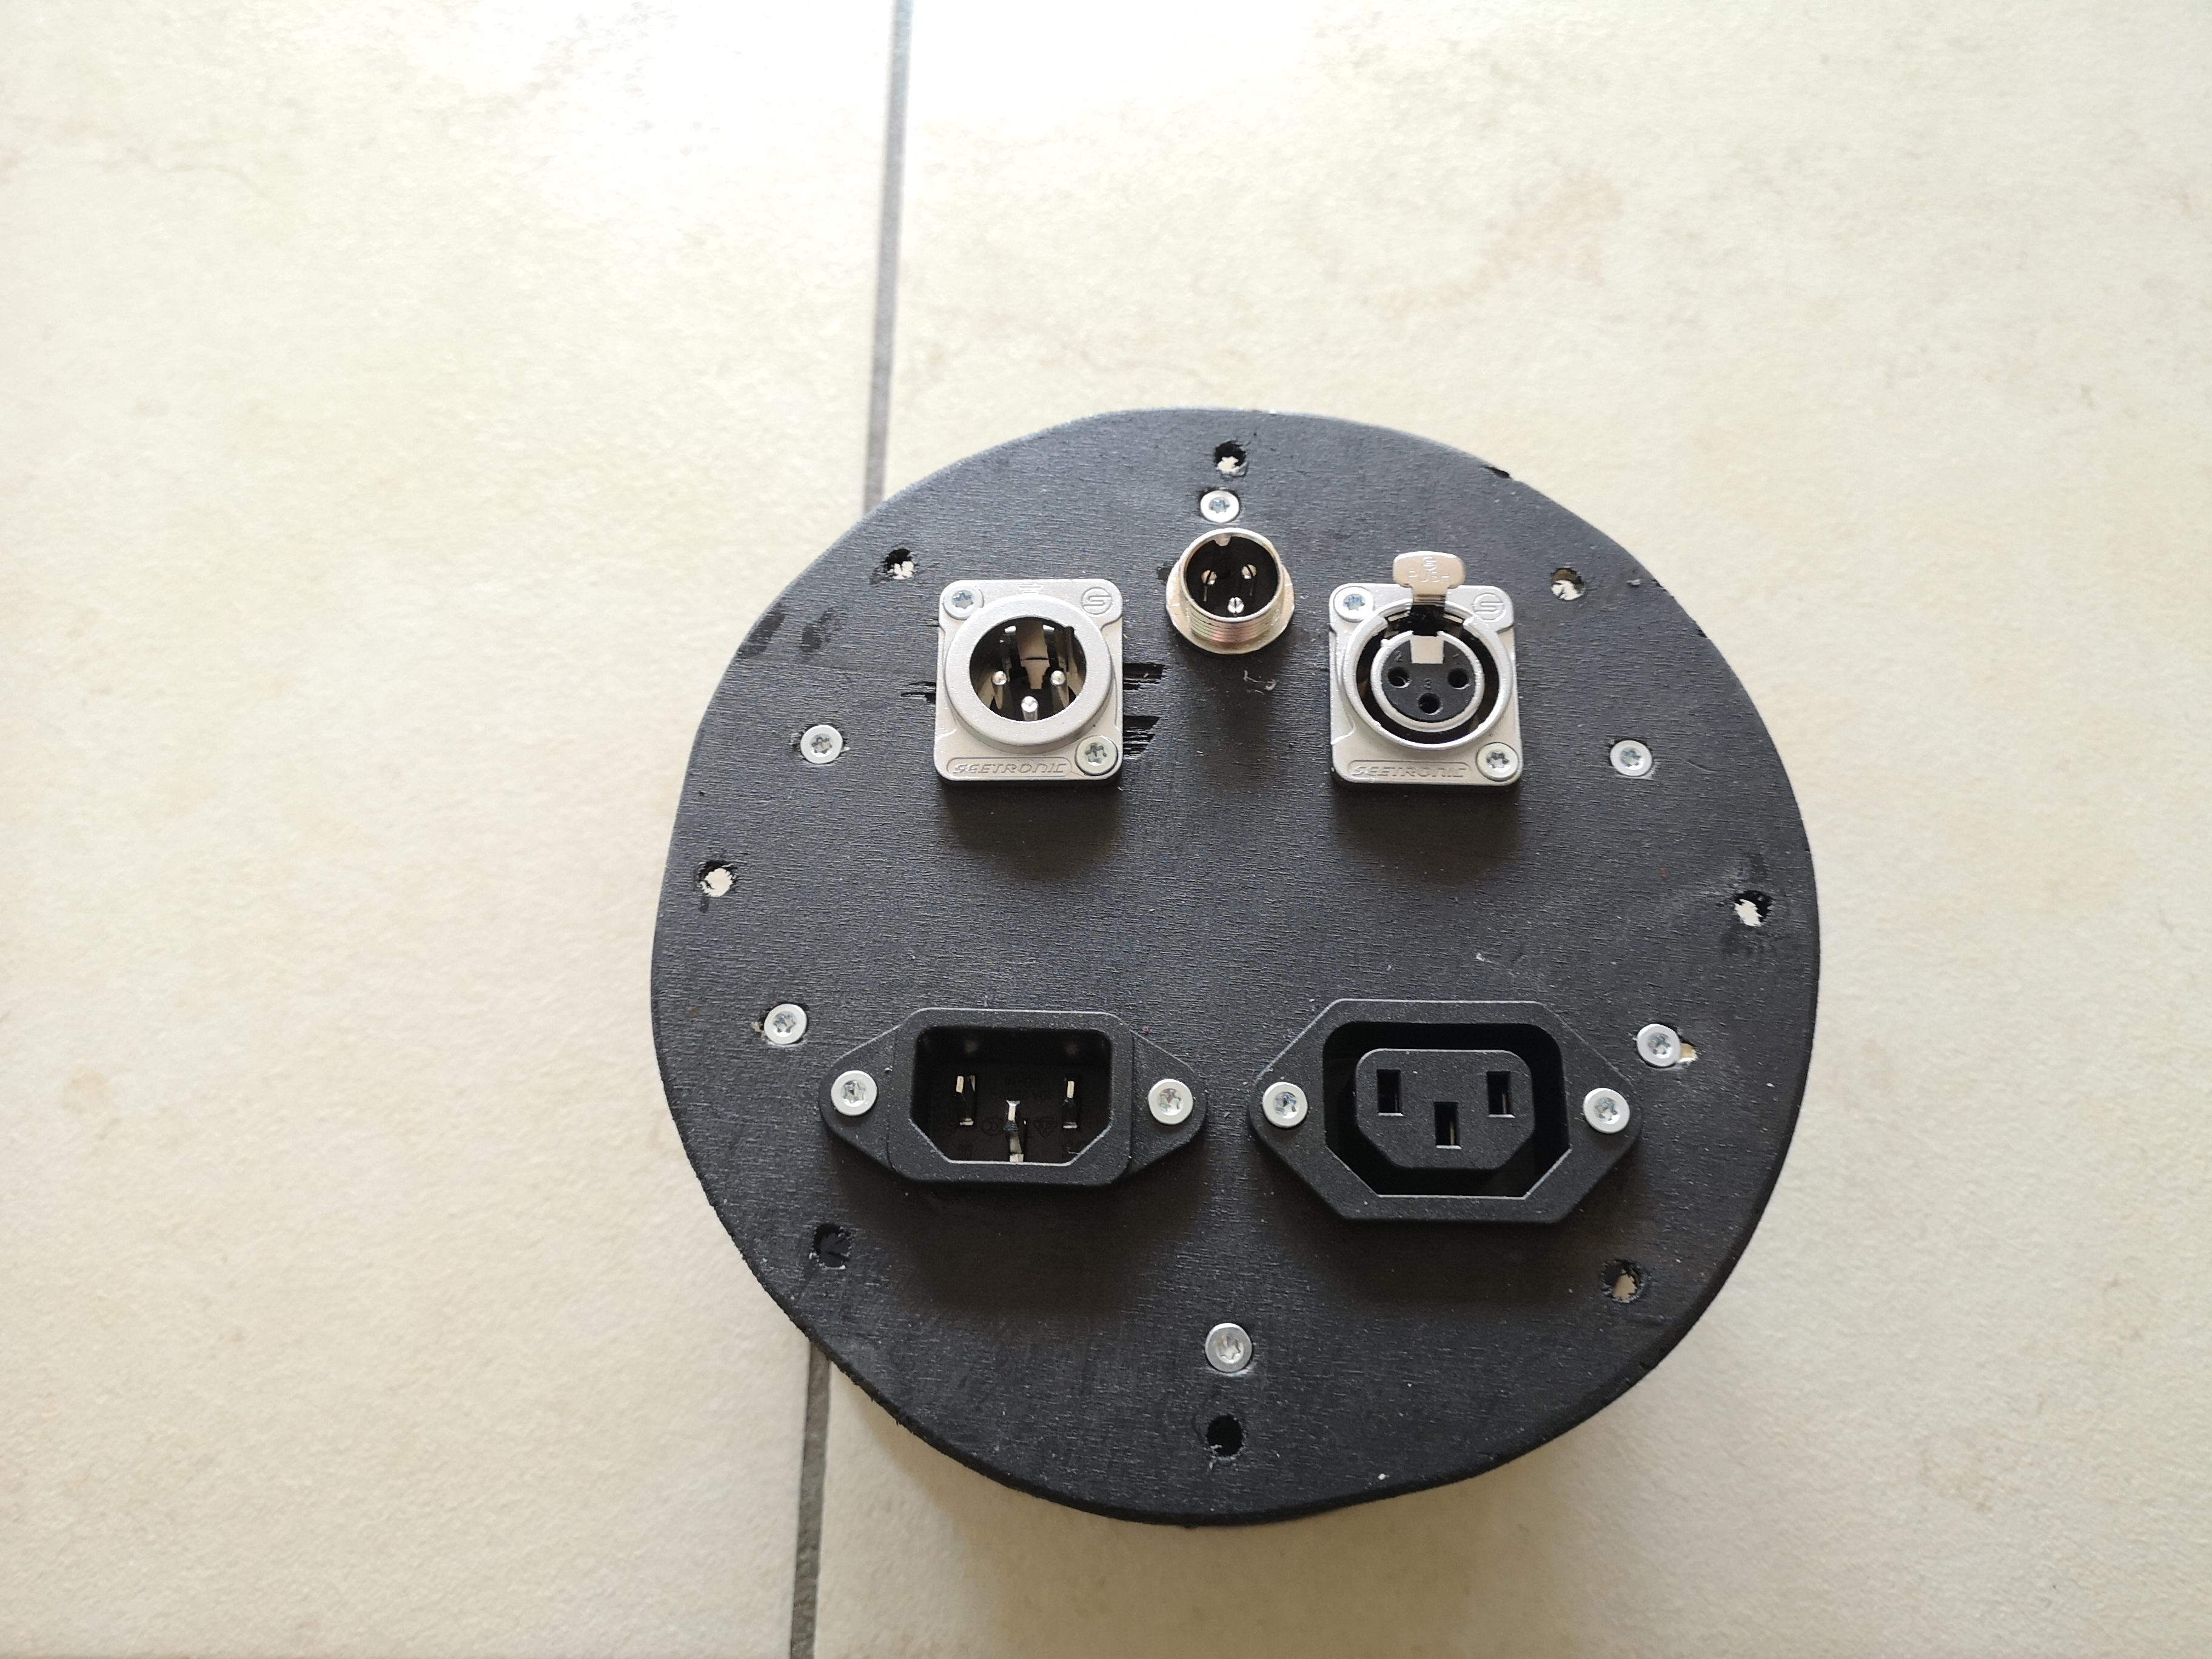
\includegraphics[width = 8.5cm]{Con-Box_front}
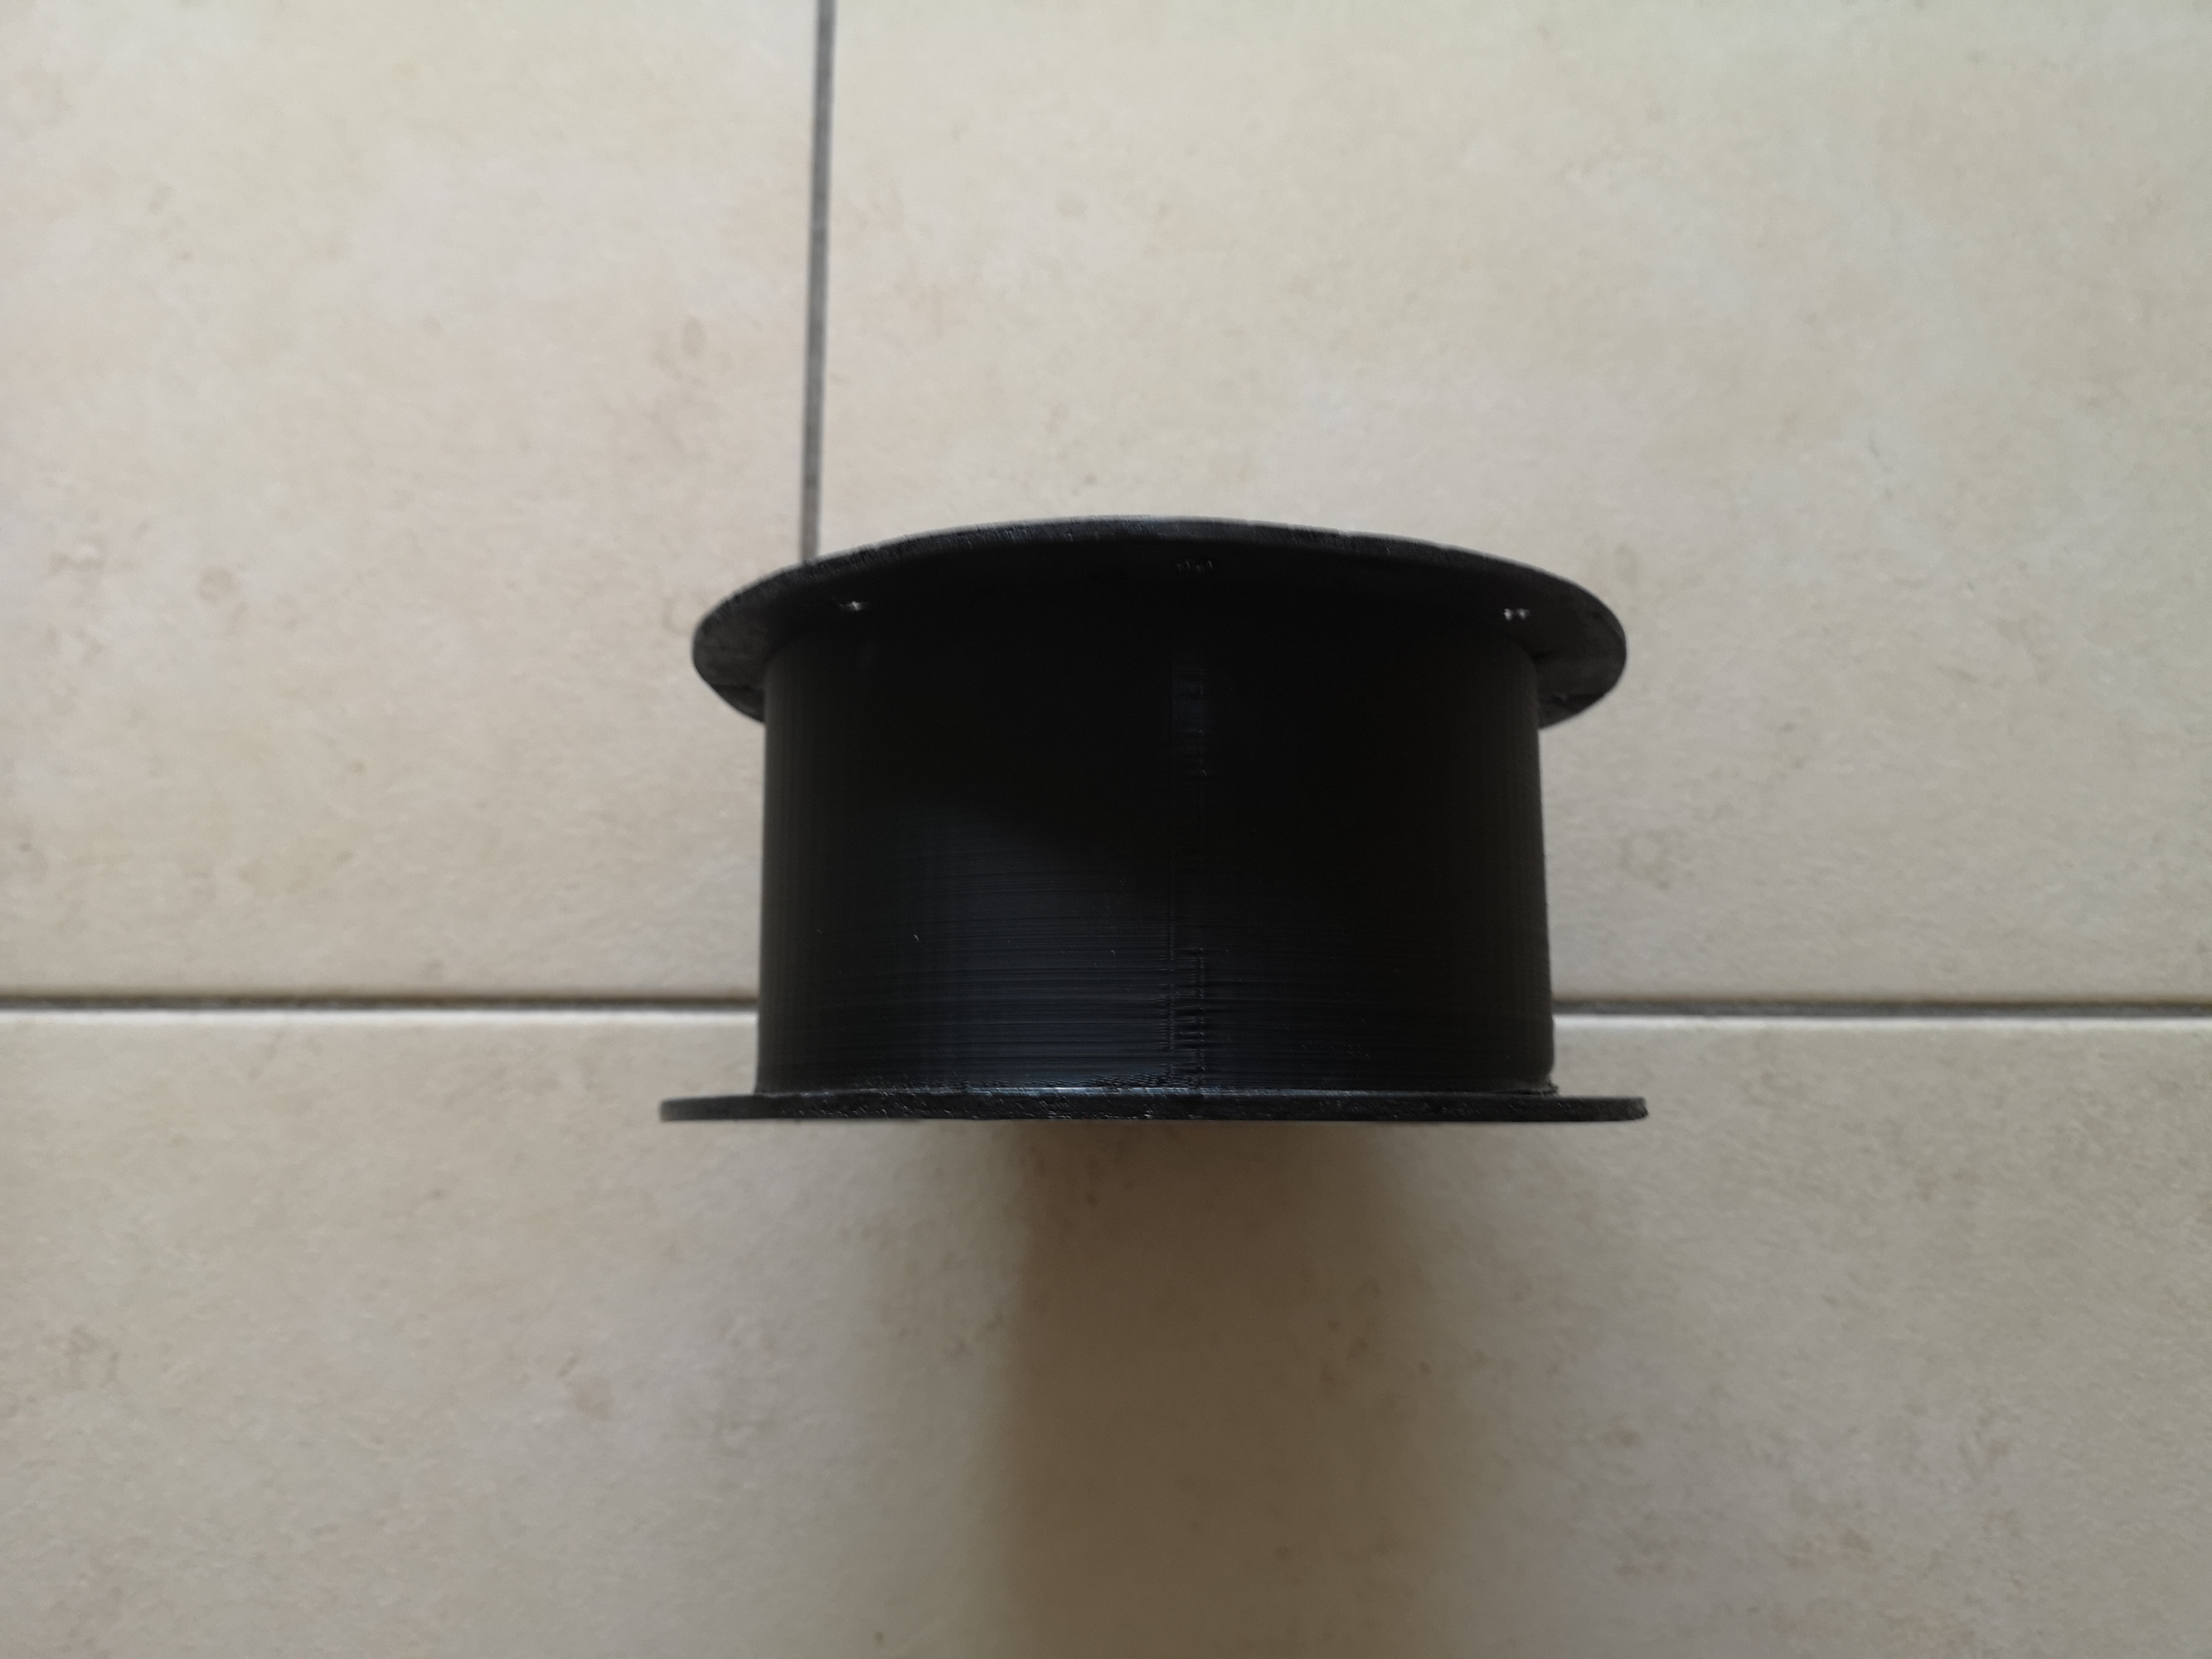
\includegraphics[width = 8.5cm]{Con-Box_side}\\
Die Anschluss-Box hat einen Durchmesser von ca. 155mm und ist ca. 70mm hoch. Auf der Rückseite befindet sich ein QR-Code der zur IP-Adresse der DMX-LED-Bar führt. \\
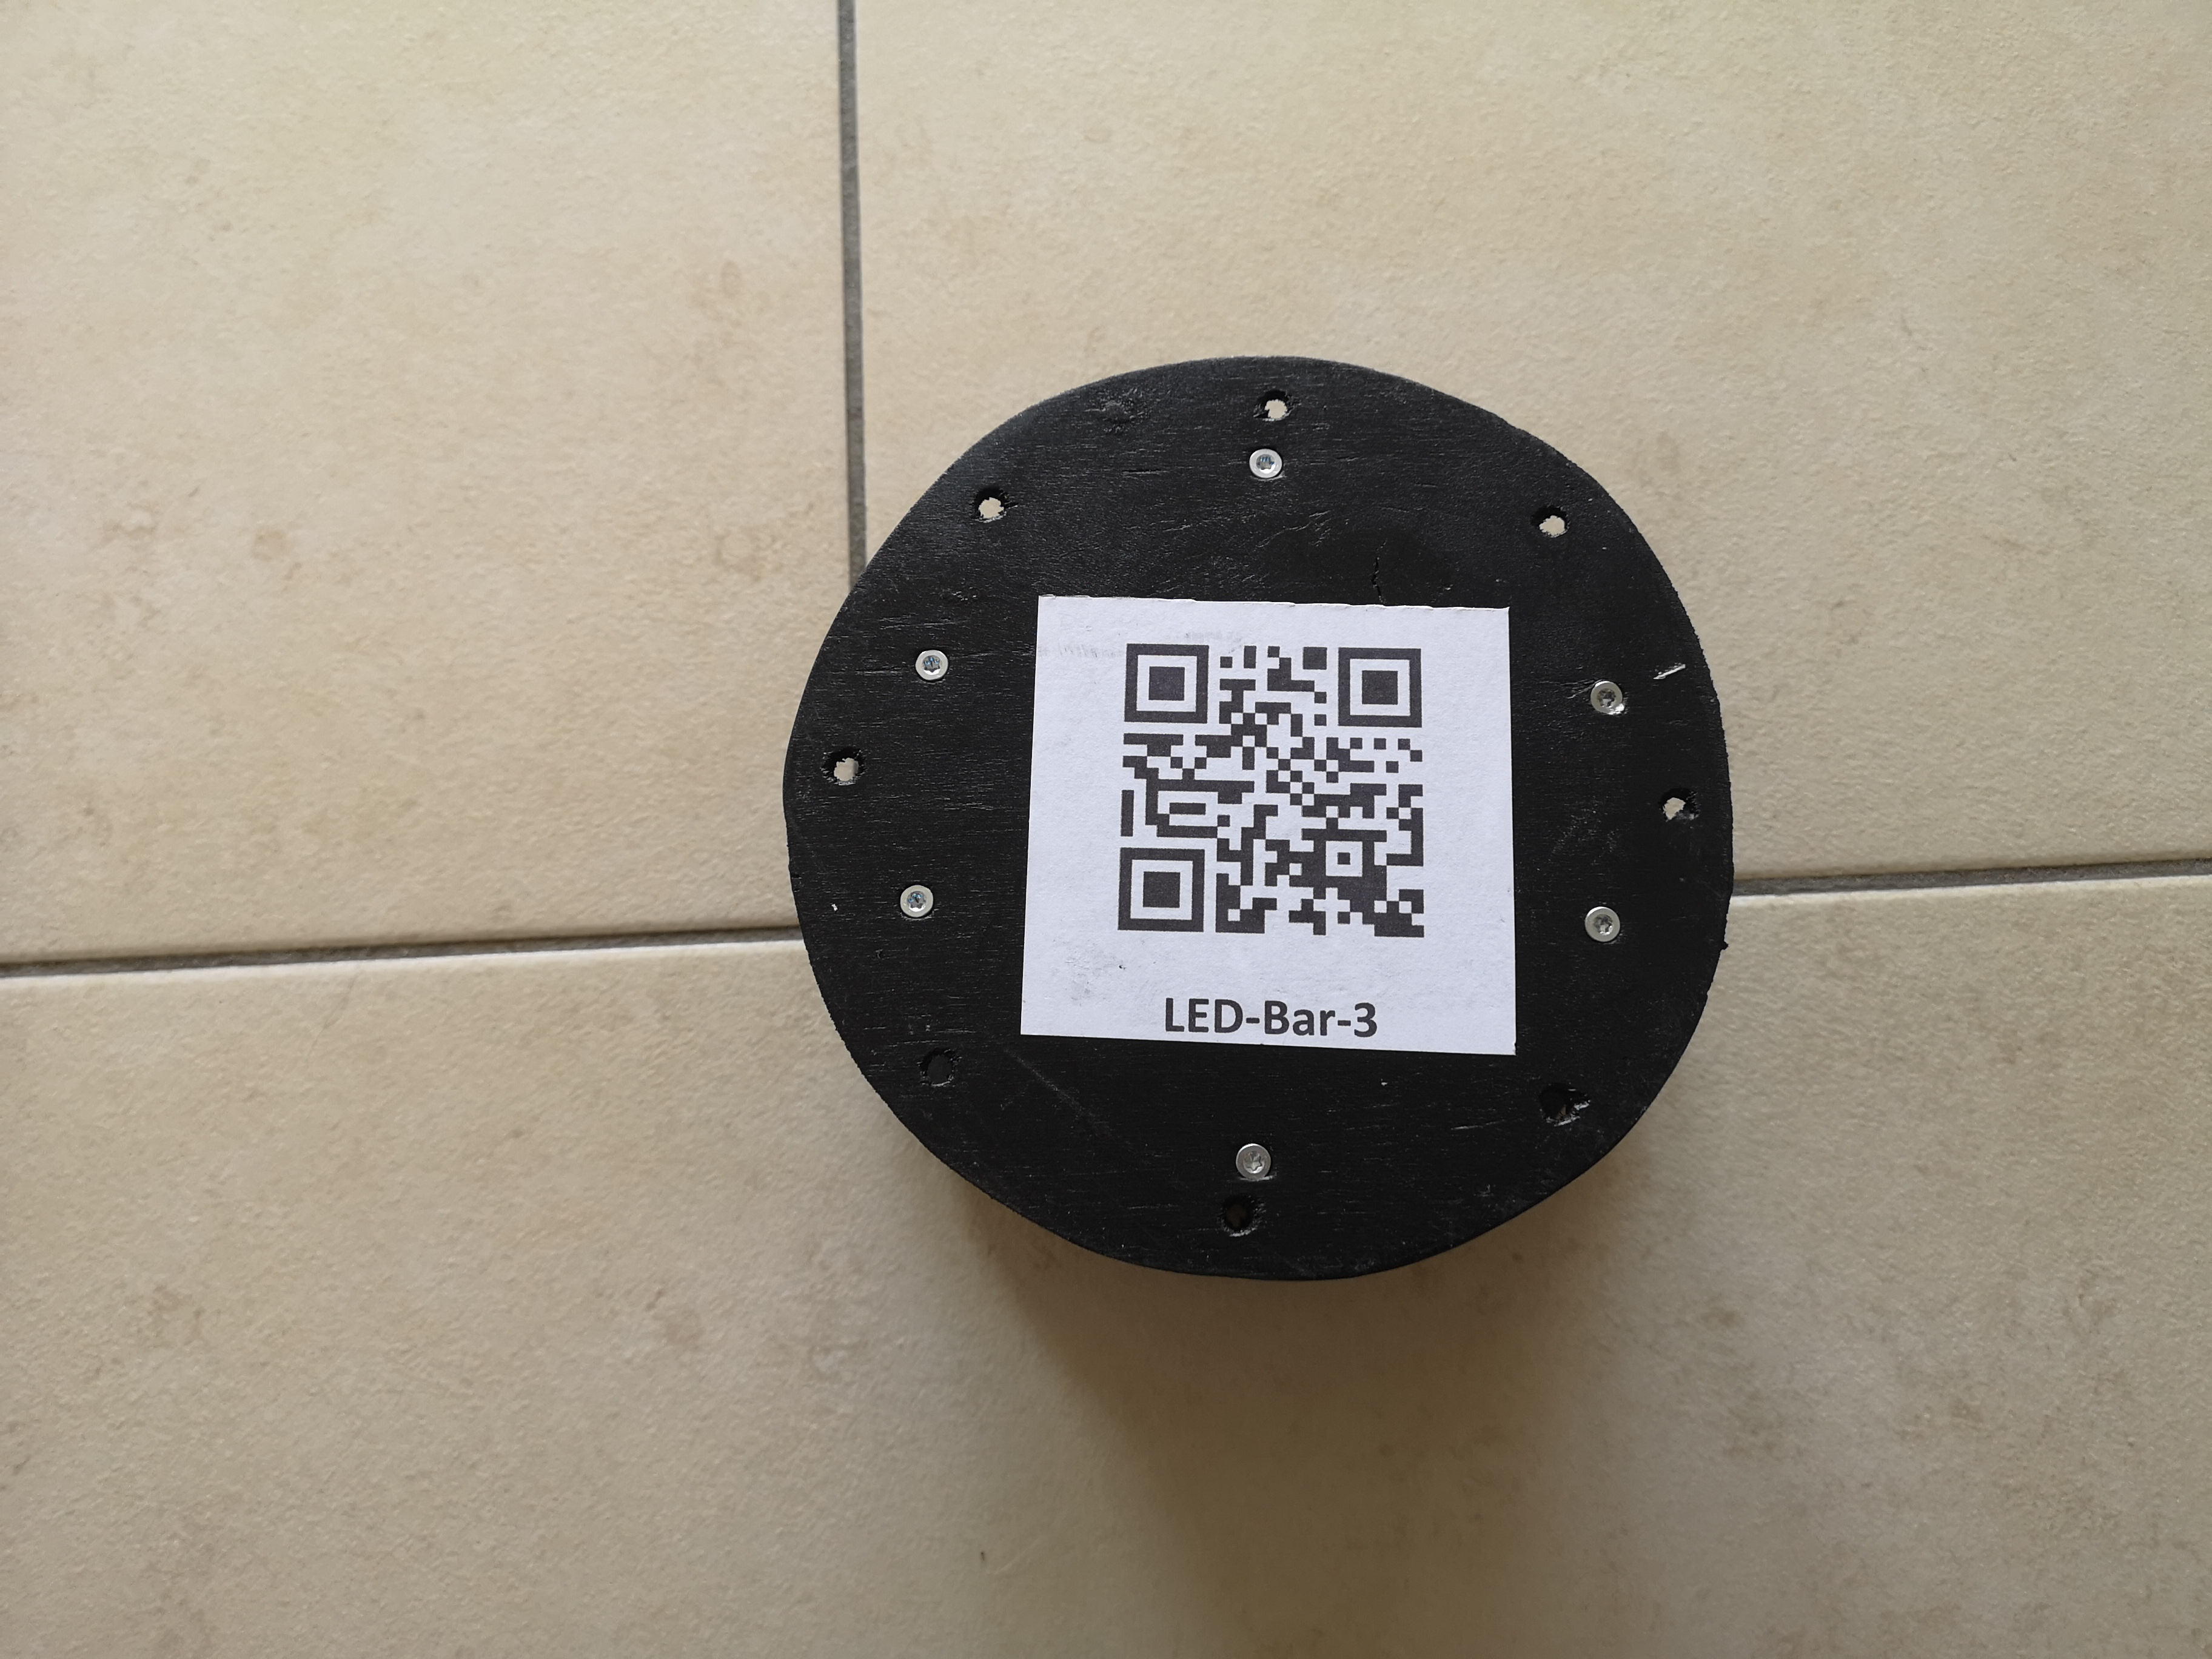
\includegraphics[width = 8.5cm]{Con-Box_back}\\
\textsuperscript{1}85-305VAC, 47-440Hz
\newpage
\section{Konfiguration}
Die DMX-LED-Bars werden über eine Website konfiguriert. Damit auf die Website zugegriffen werden kann muss sich das Konfigurationsgerät(Handy, Laptop,...) mit dem richtigen WLAN Netzwerk verbinden.
\subsection{WLAN Netzwerk}\label{WLAN Netzwerk}
Im Normalbetrieb baut die Lampe Nr. 1 (LED-Bar-1) ein, gleichnamiges, WLAN Netzwerk auf, auf welches sich das Konfigurationsgerät verbinden kann um alle 4 Bars zu konfigurieren. Dieses WLAN Netzwerk wird direkt nach dem Einschalten der LED-Bar-1 aufgeschaltet und bleibt für 10min aktiv. Um das Netzwerk länger als 10min am laufen zu halten, kann im Konfigurations-Menu der LED-Bar-1 ein Häckchen gesetzt werden, womit das Netzwerk so lange läuft bis das Häkchen wieder entfernt wird.\\
Alle anderen Bars(2-4) suchen nach dem einschalten nach dem Netzwerk von LED-Bar-1, um sich darauf zu verbinden. Sollte das Netzwerk nach 1min noch nicht gefunden worden sein, bauen alle Bars ihr eigenes WLAN Netzwerk auf. In diesem Fall muss sich das Konfigurationsgerät auf das Netzwerk der jeweiligen Bar verbinden um diese zu konfigurieren. Auch die einzelnen Netzwerke werden nach 10min wieder abgeschaltet sofern das Häckchen im Konfigurations-Menu der jeweiligen Bar nicht gesetzt wird.
\subsection{IP-Adressen}
Unabhängig davon ob sich alle Bars auf das Netzwerk von LED-Bar-1 verbinden konnten oder in ihrem eigenen Netzwerk sind, habe alle Bars immer ihre eigenen IP-Adressen:\\
LED-Bar-1: 192.168.4.1\\
LED-Bar-2: 192.168.4.12\\
LED-Bar-3: 192.168.4.13\\
LED-Bar-4: 192.168.4.14\\
Die auf den Anschluss-Boxen aufgeklebten QR-Codes führen auch zur jeweiligen IP-Adresse der Bar.
\subsection{Website}
Um die Konfigurations-Website einer Bar aufzurufen, muss mindestens: die Anschluss-Box der Bar mit Strom versorgt sein, das Konfigurationsgerät sich im richtigen WLAN Netzwerk befinden und ein Internet Browser geöffnet werden. Falls der Browser anzeigt, dass er keine Internetverbindung hat, war das zu erwarten, denn in diesem WLAN Netzwerk sind nur die Bars und das Konfigurationsgerät selbst vorhanden, aber kein Zugang zum Internet.\\
In der Adressleiste des Browsers wird die IP-Adresse der gewünschten Bar eingegeben. Zum Beispiel:\\
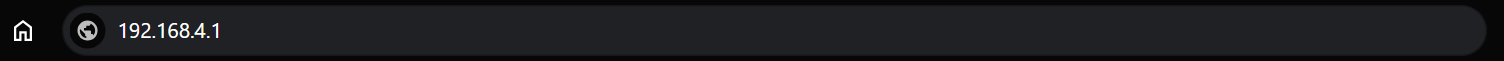
\includegraphics[width = \textwidth]{Browser_Adressleiste}\\
um sich auf die LED-Bar-1 verbinden. Danach mit Enter bestätigen. Falls man sich mit der LED-Bar-1 verbunden hat, oder mit einer Bar die ihr eigenes Netzwerk aufgebaut hat, sollte folgende Website erscheinen:\\
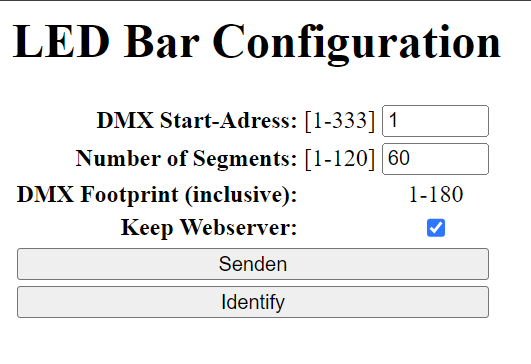
\includegraphics[width = 10cm]{Website_Main_AP}\\
Alle übertragenen Konfigurationsänderungen, ausser "Keep Webserver", bleiben auch nach Spannungsverlust erhalten und sind beim nächsten einschalten automatisch wieder in Kraft.
\subsubsection{DMX Start-Adress}
In dieses Feld wird der Anfang des Adressbereichs dieser LED-Bar eingestellt. In den Eckigen Klammern steht der zulässige Bereich. Die Obergrenze(Im Beispiel Bild: 333) ist abhängig davon wie viele Segmente man im nächsten Feld eingestellt hat. Mit dieser Obergrenze wird verhindert, dass die letzten Pixel der Bar versuchen auf DMX Kanäle zuzugreifen, die höher als 512 sind .
\subsubsection{Number of Segments}
Die 120 LED Pixel können in eine Beliebige, kleinere Anzahl Segmente unterteilt werden. Es empfiehlt sich eine Anzahl Segmente zu wählen durch welche 120 ohne Rest teilbar ist. Sollte trotzdem eine Anzahl Segmente wie z.B. 50 gefragt sein, durch welche sich 120 nicht Restlos teilen lässt, werden die hintersten Pixel dunkel bleiben.(in diesem Beispiel würden die hintersten 20 Pixel dunkel bleiben).
\subsubsection{DMX Footprint (inclusive)}
Hier wird angezeigt Welche Kanäle die Bar im DMX Netzwerk belegen wird. Im Beispiel Bild werden die Kanäle 1-180 belegt, entsprechend wäre der nächste Freie Kanal, der Kanal 181.
\subsubsection{Keep Webserver}
Das ist das Häckchen welches im Kapitel \ref{WLAN Netzwerk}(WLAN Netzwerk) erwähnt wurde. Solange dieses Häckchen gesetzt ist, bleibt das WLAN Netzwerk am laufen und die dazu verbundenen Konfigurations-Websites zugänglich. Wenn dieses Häcken nicht(mehr) gesetzt ist, und 10min seit dem Einschalten der Bar vergangen sind, wird das Nezwerk geschlossen und die Websites sind nicht mehr zugänglich bis zum nächsten Neustart der Bar(s).
\subsubsection{Button: Senden}
Erst wenn dieser Button gedrückt wird, werden die oberhalb eingetragenen Werte inkl. Häckchen an die Bar übertragen. Wenn sie aber übertragen wurden, sollten die gemachten Änderungen sofort sichtbar werden, sowohl auf der Website wie auch auf den LED Pixeln, sofern diese bereits angeschlossen sind.
\subsubsection{Button: Identify}
Wenn dieser Button gedrückt wird, wird was auch immer zuvor angezeigt wurde unterbrochen und ein Identifizierungs Muster gespielt: Die ganze LED-Bar bilnkt einmal rot, grün, blau. Auch wenn während dem Identifizierungs Muster weitere DMX Daten ankommen, werden diese ignoriert bis das ca. 1 Sekündige Muster durchgelaufen ist. Diese Funktion kann genutzt werden, wenn nicht mehr klar ist welche bar wo verbaut worden ist.
\subsubsection{Website der Bars 2-4 im Netz von LED-Bar1}
Wenn sich auf die Konfigurationsseite einer anderen Bar verbunden wird, als LED-Bar-1 aber über das WLAN Netzwerk von LED-Bar-1, dann sieht die Website minim anders aus:\\
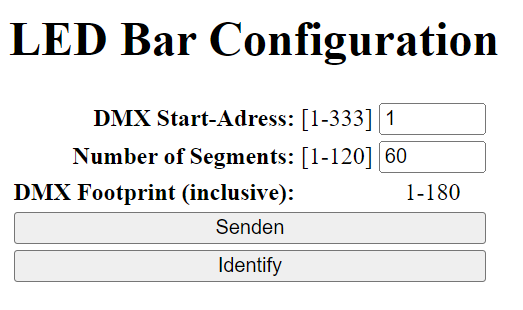
\includegraphics[width = 10cm]{Website_Non_Main_AP}\\ 
Es fehlt das Häckchen "Keep Webserver" dieses existiert nur wenn eine Bar ein eigenes WLAN Netzwerk hat, was im Normalfall nur die LED-Bar-1 ist. Ansonsten funktioniert die Konfiguration genau gleich wie oben beschrieben. 
\end{document}

